% !TEX TS-program = pdflatex
\documentclass[11pt]{article}

% -------------------- Packages --------------------
\usepackage[a4paper,margin=1in]{geometry}
\usepackage{amsmath,amssymb}
\usepackage[T1]{fontenc}
\usepackage{lmodern}
\usepackage{xcolor}
\usepackage{tcolorbox}
\tcbuselibrary{skins,breakable}
\usepackage{enumitem}
\usepackage{hyperref}
\usepackage{tikz}
\usetikzlibrary{calc,angles,quotes,arrows.meta}

\pagestyle{empty}

% -------------------- Dark Theme Colors --------------------
\definecolor{bg}{HTML}{000000}
\definecolor{pairbg}{HTML}{121212}
\definecolor{solbg}{HTML}{0A0A0A}
\definecolor{border}{HTML}{2A2A2A}
\definecolor{text}{HTML}{FFFFFF}
\definecolor{muted}{HTML}{C9CDD3}
\definecolor{gold}{HTML}{FFD700}
\definecolor{green}{HTML}{4ADE80}
\definecolor{cyan}{HTML}{38BDF8}

\pagecolor{bg}
\color{text}

\hypersetup{
  colorlinks=true,
  linkcolor=cyan,
  urlcolor=cyan
}

\setlength{\parindent}{0pt}
\setlength{\parskip}{10pt}

% Help LaTeX avoid overfull lines globally
\sloppy
\setlength{\emergencystretch}{3em}

\setlist[itemize]{left=1.4em,itemsep=6pt,topsep=6pt}
\setlist[enumerate]{left=1.6em,itemsep=4pt,topsep=4pt}

% -------------------- tcolorbox Base --------------------
\tcbset{
  enhanced,
  breakable,
  arc=12pt,
  boxrule=0.8pt,
  left=14pt,right=14pt,top=12pt,bottom=12pt
}

\newtcolorbox{QAPair}[1]{%
  colback=pairbg,
  colbacklower=solbg,
  colframe=border,
  coltext=text,
  title=\textcolor{gold}{\bfseries #1},
  fonttitle=\bfseries,
  coltitle=text,
  segmentation style={draw=border, dashed, line width=0.6pt},
  before upper=\raggedright,
  before lower=\raggedright
}

\newtcolorbox{QuickBox}{%
  colback=pairbg,
  colframe=cyan,
  coltext=text,
  fontupper=\color{text}\raggedright,
  borderline north={4pt}{0pt}{cyan},
  arc=14pt,
  boxrule=0.8pt
}

% Helper for step headings
\newcommand{\Step}[1]{\textcolor{muted}{\textbf{Step #1:}}}

% Small centered diagram block
\newenvironment{StepDiagram}{\par\medskip\begin{center}}{\end{center}\medskip}

% TikZ styles
\tikzset{
  base/.style={draw=text, line width=0.9pt, line cap=round, line join=round},
  new/.style={draw=cyan, line width=1.2pt, line cap=round, line join=round},
  help/.style={draw=muted, dashed, line width=0.9pt},
  ang/.style={draw=gold, line width=1.0pt},
  dot/.style={circle, fill=text, inner sep=1.2pt},
  lab/.style={text=text, font=\small},
  labm/.style={text=muted, font=\small},
}

% Compact callout (safe for mixed text+math)
\newcommand{\EqDiagram}[1]{%
\begin{StepDiagram}
\begin{tikzpicture}
\node[
  draw=border,
  rounded corners=10pt,
  inner sep=8pt,
  text=text,
  align=left
]{
  \begin{minipage}{0.85\linewidth}
  \color{text}#1
  \end{minipage}
};
\end{tikzpicture}
\end{StepDiagram}
}

% ============================================================
\begin{document}

\begin{center}
{\LARGE\bfseries \textcolor{gold}{Miscellaneous Exercise 11 --- Solutions}}\\[-2pt]
\end{center}

% -------------------- Quick facts (each line has its own diagram) --------------------
\begin{QuickBox}
{\color{cyan}\bfseries Quick facts used (Tangents \& Circles)}\par\medskip

\begin{itemize}

\item \textbf{Radius $\perp$ tangent at point of contact.}
\begin{StepDiagram}
\begin{tikzpicture}[scale=1.0]
  \def\r{1.8}
  \coordinate (O) at (0,0);
  \coordinate (P) at (40:\r);
  \coordinate (T1) at ($(P)+({-1.7*sin(40)},{ 1.7*cos(40)})$);
  \coordinate (T2) at ($(P)+({ 1.7*sin(40)},{-1.7*cos(40)})$);

  \draw[base] (O) circle (\r);
  \node[dot,label={[lab]below:$O$}] at (O) {};
  \node[dot,label={[lab]right:$P$}] at (P) {};
  \draw[new] (O)--(P);
  \draw[new] (T1)--(T2);

  % right angle mark at P
  \draw[base] ($(P)+(-0.16,0)$) -- ($(P)+(-0.16,-0.16)$) -- ($(P)+(0,-0.16)$);
  \node[labm] at (0,-2.15) {$OP \perp$ tangent at $P$};
\end{tikzpicture}
\end{StepDiagram}

\item \textbf{Touching circles: external and internal.}
\[
\text{External touch: } PQ=r_1+r_2,\qquad
\text{Internal touch: } PQ=\lvert r_1-r_2\rvert.
\]

% External touch diagram
\begin{StepDiagram}
\begin{tikzpicture}[scale=0.95]
  \coordinate (P) at (0,0);
  \coordinate (Q) at (3.3,0);
  \def\rA{1.2}
  \def\rB{2.1}
  \draw[base] (P) circle (\rA);
  \draw[base] (Q) circle (\rB);
  \node[dot,label={[lab]below:$P$}] at (P) {};
  \node[dot,label={[lab]below:$Q$}] at (Q) {};
  \draw[new] (P)--(Q);
  \node[lab, fill=pairbg, inner sep=1.2pt] at ($(P)!0.35!(Q)$) {$r_1$};
  \node[lab, fill=pairbg, inner sep=1.2pt] at ($(P)!0.72!(Q)$) {$r_2$};
  \node[labm] at (1.65,-2.55) {External touch $\Rightarrow PQ=r_1+r_2$};
\end{tikzpicture}
\end{StepDiagram}

% Internal touch diagram
\begin{StepDiagram}
\begin{tikzpicture}[scale=0.95]
  \coordinate (Q) at (0,0);
  \def\rB{2.2}
  \def\rA{1.4}
  \coordinate (P) at (0.8,0); % inside
  \draw[base] (Q) circle (\rB);
  \draw[base] (P) circle (\rA);
  \node[dot,label={[lab]below:$Q$}] at (Q) {};
  \node[dot,label={[lab]below:$P$}] at (P) {};
  \draw[new] (Q)--(P);
  \node[labm] at (0,-2.75) {Internal touch $\Rightarrow PQ=\lvert r_2-r_1\rvert$};
\end{tikzpicture}
\end{StepDiagram}

\item \textbf{Square and circle:} incircle in square of side $s$ has $r=\dfrac{s}{2}$;\;
square in circle of radius $r$ has diagonal $=2r$.

% Incircle in square
\begin{StepDiagram}
\begin{tikzpicture}[scale=0.95]
  \coordinate (A) at (-1.8,-1.8);
  \coordinate (B) at ( 1.8,-1.8);
  \coordinate (C) at ( 1.8, 1.8);
  \coordinate (D) at (-1.8, 1.8);
  \coordinate (O) at (0,0);
  \draw[base] (A)--(B)--(C)--(D)--cycle;
  \draw[base] (O) circle (1.8);
  \node[dot,label={[lab]below:$O$}] at (O) {};
  \node[labm] at (0,-2.55) {Incircle: $2r=s \Rightarrow r=\frac{s}{2}$};
\end{tikzpicture}
\end{StepDiagram}

% Square in circle
\begin{StepDiagram}
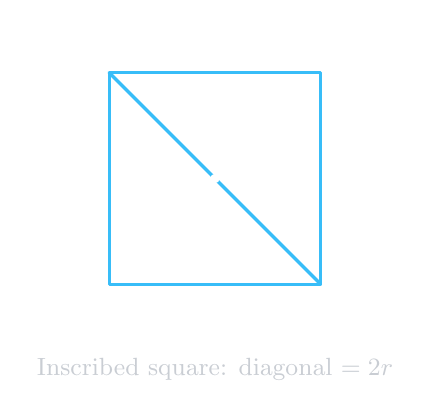
\begin{tikzpicture}[scale=0.95]
  \def\r{2.0}
  \coordinate (O) at (0,0);
  \coordinate (A) at (45:\r);
  \coordinate (B) at (135:\r);
  \coordinate (C) at (225:\r);
  \coordinate (D) at (315:\r);
  \draw[base] (O) circle (\r);
  \draw[new] (A)--(B)--(C)--(D)--cycle;
  \draw[new] (B)--(D); % diagonal
  \node[dot,label={[lab]below:$O$}] at (O) {};
  \node[labm] at (0,-2.55) {Inscribed square: diagonal $=2r$};
\end{tikzpicture}
\end{StepDiagram}

\item \textbf{Chord fact:} Perpendicular bisector of a chord passes through the centre.

\begin{StepDiagram}
\begin{tikzpicture}[scale=1.0]
  \def\r{2.0}
  \coordinate (O) at (0,0);
  \coordinate (A) at (210:\r);
  \coordinate (B) at (330:\r);
  \coordinate (M) at ($(A)!0.5!(B)$);
  \draw[base] (O) circle (\r);
  \draw[new] (A)--(B);
  \draw[help] (M) -- ($(M)!1.4!(O)$);
  \draw[help] (M) -- ($(M)!1.4!(-O)$);
  \node[dot,label={[lab]below:$O$}] at (O) {};
  \node[dot,label={[lab]left:$A$}] at (A) {};
  \node[dot,label={[lab]right:$B$}] at (B) {};
  \node[dot,label={[lab]below:$M$}] at (M) {};
  \node[labm] at (0,-2.55) {Perpendicular bisector of chord $AB$ passes through $O$};
\end{tikzpicture}
\end{StepDiagram}

\end{itemize}
\end{QuickBox}

% ============================================================
% Q1(i)
\begin{QAPair}{Question 1 (i)}
\textcolor{gold}{\bfseries Question:} Angle between tangent and radial segment of a circle is:
(a) $30^\circ$ \ (b) $45^\circ$ \ (c) $60^\circ$ \ (d) $90^\circ$.
\tcblower
\textcolor{green}{\bfseries Answer:}\par

\Step{1} Radius at the point of contact is perpendicular to the tangent.

\begin{StepDiagram}
\begin{tikzpicture}[scale=0.95]
  \def\r{1.9}
  \coordinate (O) at (0,0);
  \coordinate (P) at (25:\r);
  \coordinate (T1) at ($(P)+({-2.0*sin(25)},{ 2.0*cos(25)})$);
  \coordinate (T2) at ($(P)+({ 2.0*sin(25)},{-2.0*cos(25)})$);
  \draw[base] (O) circle (\r);
  \draw[new] (O)--(P);
  \draw[new] (T1)--(T2);
  \node[dot,label={[lab]below:$O$}] at (O) {};
  \node[dot,label={[lab]right:$P$}] at (P) {};
\end{tikzpicture}
\end{StepDiagram}

\Step{2} Therefore the angle is $90^\circ$.

\begin{StepDiagram}
\begin{tikzpicture}[scale=0.95]
  \def\r{1.9}
  \coordinate (O) at (0,0);
  \coordinate (P) at (25:\r);
  \coordinate (T1) at ($(P)+({-2.0*sin(25)},{ 2.0*cos(25)})$);
  \coordinate (T2) at ($(P)+({ 2.0*sin(25)},{-2.0*cos(25)})$);
  \draw[base] (O) circle (\r);
  \draw[new] (O)--(P);
  \draw[new] (T1)--(T2);
  \draw[base] ($(P)+(-0.16,0)$) -- ($(P)+(-0.16,-0.16)$) -- ($(P)+(0,-0.16)$);
  \node[lab, fill=pairbg, inner sep=1.2pt] at ($(P)+(0.55,0.35)$) {$90^\circ$};
\end{tikzpicture}
\end{StepDiagram}

\[
\boxed{\textcolor{green}{(d)\ 90^\circ}}
\]
\end{QAPair}

% ============================================================
% Q1(ii)
\begin{QAPair}{Question 1 (ii)}
\textcolor{gold}{\bfseries Question:} Direct common tangents of equal circles are:
(a) parallel \ (b) intersecting \ (c) converging \ (d) not parallel.
\tcblower
\textcolor{green}{\bfseries Answer:}\par

\Step{1} For two equal circles, the two \emph{direct} (external) common tangents keep the same separation.

\begin{StepDiagram}
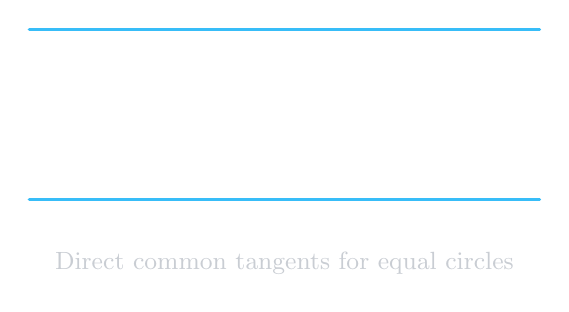
\begin{tikzpicture}[scale=0.9]
  \def\r{1.2}
  \coordinate (O1) at (-2.0,0);
  \coordinate (O2) at ( 2.0,0);
  \draw[base] (O1) circle (\r);
  \draw[base] (O2) circle (\r);
  % direct tangents (top and bottom)
  \draw[new] (-3.6, \r) -- (3.6, \r);
  \draw[new] (-3.6,-\r) -- (3.6,-\r);
  \node[dot,label={[lab]below:$O_1$}] at (O1) {};
  \node[dot,label={[lab]below:$O_2$}] at (O2) {};
  \node[labm] at (0,-2.1) {Direct common tangents for equal circles};
\end{tikzpicture}
\end{StepDiagram}

\Step{2} Hence they are parallel.

\begin{StepDiagram}
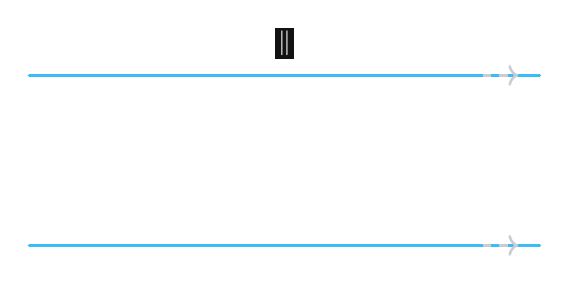
\begin{tikzpicture}[scale=0.9]
  \def\r{1.2}
  \coordinate (O1) at (-2.0,0);
  \coordinate (O2) at ( 2.0,0);
  \draw[base] (O1) circle (\r);
  \draw[base] (O2) circle (\r);
  \draw[new] (-3.6, \r) -- (3.6, \r);
  \draw[new] (-3.6,-\r) -- (3.6,-\r);
  \draw[help,->] (2.8,\r) -- (3.3,\r);
  \draw[help,->] (2.8,-\r) -- (3.3,-\r);
  \node[lab, fill=pairbg, inner sep=1.2pt] at (0,1.65) {$\parallel$};
\end{tikzpicture}
\end{StepDiagram}

\[
\boxed{\textcolor{green}{(a)\ parallel}}
\]
\end{QAPair}

% ============================================================
% Q1(iii)
\begin{QAPair}{Question 1 (iii)}
\textcolor{gold}{\bfseries Question:} How many tangents can be drawn to two intersecting circles?
(a) $1$ \ (b) $2$ \ (c) $3$ \ (d) infinite.
\tcblower
\textcolor{green}{\bfseries Answer:}\par

\Step{1} Two circles intersect $\Rightarrow$ only two \emph{external} common tangents exist.

\begin{StepDiagram}
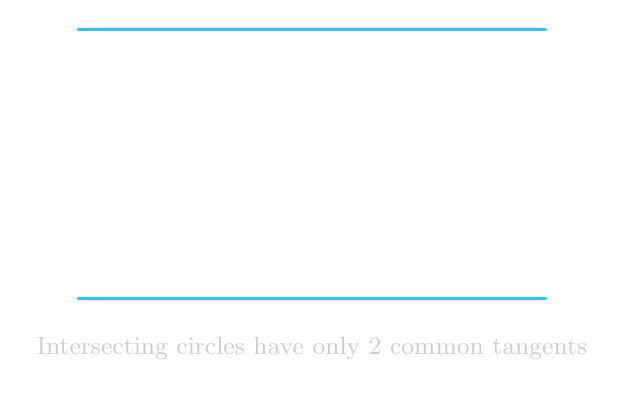
\begin{tikzpicture}[scale=0.9]
  \def\r{1.5}
  \coordinate (O1) at (-1.3,0);
  \coordinate (O2) at ( 1.3,0);
  \draw[base] (O1) circle (\r);
  \draw[base] (O2) circle (\r);
  % external tangents (approx)
  \draw[new] (-3.3, 1.9) -- (3.3, 1.9);
  \draw[new] (-3.3,-1.9) -- (3.3,-1.9);
  \node[dot,label={[lab]below:$O_1$}] at (O1) {};
  \node[dot,label={[lab]below:$O_2$}] at (O2) {};
  \node[labm] at (0,-2.6) {Intersecting circles have only 2 common tangents};
\end{tikzpicture}
\end{StepDiagram}

\Step{2} So the number is $2$.

\begin{StepDiagram}
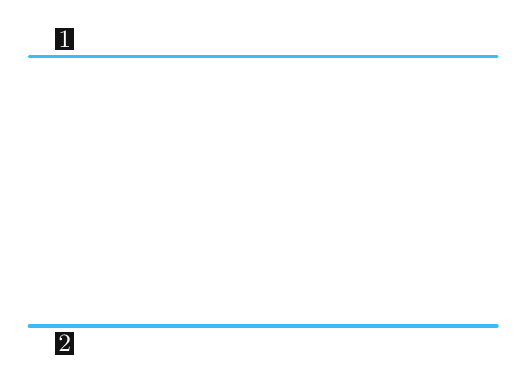
\begin{tikzpicture}[scale=0.9]
  \def\r{1.5}
  \coordinate (O1) at (-1.3,0);
  \coordinate (O2) at ( 1.3,0);
  \draw[base] (O1) circle (\r);
  \draw[base] (O2) circle (\r);
  \draw[new] (-3.3, 1.9) -- (3.3, 1.9);
  \draw[new] (-3.3,-1.9) -- (3.3,-1.9);
  \node[lab, fill=pairbg, inner sep=1.2pt] at (-2.8,2.15) {$1$};
  \node[lab, fill=pairbg, inner sep=1.2pt] at (-2.8,-2.15) {$2$};
\end{tikzpicture}
\end{StepDiagram}

\[
\boxed{\textcolor{green}{(b)\ 2}}
\]
\end{QAPair}

% ============================================================
% Q1(iv)
\begin{QAPair}{Question 1 (iv)}
\textcolor{gold}{\bfseries Question:} Two circles having radii $3$ cm and $3.2$ cm touch externally.
The distance between centres is:
(a) $6$ cm \ (b) $0.2$ cm \ (c) $6.2$ cm \ (d) $5.3$ cm.
\tcblower
\textcolor{green}{\bfseries Answer:}\par

\Step{1} External touch $\Rightarrow$ distance between centres $=r_1+r_2$.

\begin{StepDiagram}
\begin{tikzpicture}[scale=0.9]
  \coordinate (O1) at (0,0);
  \coordinate (O2) at (3.9,0);
  \def\rA{1.5}
  \def\rB{2.4}
  \draw[base] (O1) circle (\rA);
  \draw[base] (O2) circle (\rB);
  \node[dot,label={[lab]below:$O_1$}] at (O1) {};
  \node[dot,label={[lab]below:$O_2$}] at (O2) {};
  \draw[new] (O1)--(O2);
  \node[labm] at (1.95,-2.9) {External touch: $O_1O_2=r_1+r_2$};
\end{tikzpicture}
\end{StepDiagram}

\Step{2} $3+3.2=6.2$ cm.

\begin{StepDiagram}
\begin{tikzpicture}[scale=0.9]
  \coordinate (O1) at (0,0);
  \coordinate (O2) at (3.9,0);
  \def\rA{1.5}
  \def\rB{2.4}
  \draw[base] (O1) circle (\rA);
  \draw[base] (O2) circle (\rB);
  \draw[new] (O1)--(O2);
  \node[lab, fill=pairbg, inner sep=1.2pt] at ($(O1)!0.5!(O2)$) {$6.2$};
\end{tikzpicture}
\end{StepDiagram}

\[
\boxed{\textcolor{green}{(c)\ 6.2\text{ cm}}}
\]
\end{QAPair}

% ============================================================
% Q1(v)
\begin{QAPair}{Question 1 (v)}
\textcolor{gold}{\bfseries Question:} Centres and point of contact of two touching circles are:
(a) collinear \ (b) non-collinear \ (c) converging \ (d) coincident.
\tcblower
\textcolor{green}{\bfseries Answer:}\par

\Step{1} The point of contact lies on the line joining the two centres.

\begin{StepDiagram}
\begin{tikzpicture}[scale=0.9]
  \coordinate (O1) at (0,0);
  \coordinate (O2) at (4,0);
  \def\rA{1.5}
  \def\rB{2.5}
  \coordinate (T) at (1.5,0); % approximate touch point along line
  \draw[base] (O1) circle (\rA);
  \draw[base] (O2) circle (\rB);
  \draw[new] (O1)--(O2);
  \node[dot,label={[lab]below:$O_1$}] at (O1) {};
  \node[dot,label={[lab]below:$O_2$}] at (O2) {};
  \node[dot,label={[lab]below:$T$}] at (T) {};
\end{tikzpicture}
\end{StepDiagram}

\Step{2} Hence they are collinear.

\begin{StepDiagram}
\begin{tikzpicture}[scale=0.9]
  \coordinate (O1) at (0,0);
  \coordinate (O2) at (4,0);
  \def\rA{1.5}
  \def\rB{2.5}
  \coordinate (T) at (1.5,0);
  \draw[base] (O1) circle (\rA);
  \draw[base] (O2) circle (\rB);
  \draw[new] (O1)--(O2);
  \node[lab, fill=pairbg, inner sep=1.2pt] at (2,0.35) {collinear};
\end{tikzpicture}
\end{StepDiagram}

\[
\boxed{\textcolor{green}{(a)\ collinear}}
\]
\end{QAPair}

% ============================================================
% Q1(vi)
\begin{QAPair}{Question 1 (vi)}
\textcolor{gold}{\bfseries Question:} In which type of triangle, incenter and circumcenter are coincident?
(a) scalene \ (b) isosceles \ (c) equilateral \ (d) right triangle.
\tcblower
\textcolor{green}{\bfseries Answer:}\par

\Step{1} Only an equilateral triangle has all centres at the same point.

\begin{StepDiagram}
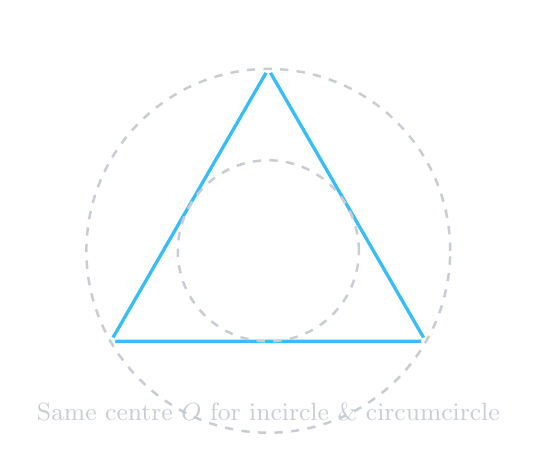
\begin{tikzpicture}[scale=1.0]
  \coordinate (A) at (-2,0);
  \coordinate (B) at ( 2,0);
  \coordinate (C) at (0,3.46);
  \coordinate (O) at (0,1.15);
  \draw[new] (A)--(B)--(C)--cycle;
  \node[dot,label={[lab]below:$A$}] at (A) {};
  \node[dot,label={[lab]below:$B$}] at (B) {};
  \node[dot,label={[lab]above:$C$}] at (C) {};
  \node[dot,label={[lab]right:$O$}] at (O) {};
  \draw[help] (O) circle (2.31); % circumcircle (approx)
  \draw[help] (O) circle (1.15); % incircle (approx)
  \node[labm] at (0,-0.9) {Same centre $O$ for incircle \& circumcircle};
\end{tikzpicture}
\end{StepDiagram}

\Step{2} Hence the triangle is equilateral.

\begin{StepDiagram}
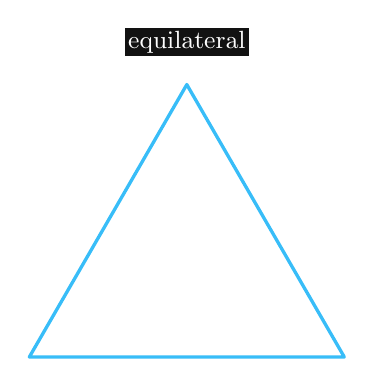
\begin{tikzpicture}[scale=1.0]
  \coordinate (A) at (-2,0);
  \coordinate (B) at ( 2,0);
  \coordinate (C) at (0,3.46);
  \coordinate (O) at (0,1.15);
  \draw[new] (A)--(B)--(C)--cycle;
  \node[dot,label={[lab]right:$O$}] at (O) {};
  \node[lab, fill=pairbg, inner sep=1.2pt] at (0,4.0) {equilateral};
\end{tikzpicture}
\end{StepDiagram}

\[
\boxed{\textcolor{green}{(c)\ equilateral}}
\]
\end{QAPair}

% ============================================================
% Q1(vii)
\begin{QAPair}{Question 1 (vii)}
\textcolor{gold}{\bfseries Question:} Two circles with radii $4$ cm and $4.8$ cm touch internally.
The distance between centres is:
(a) $4$ cm \ (b) $8$ cm \ (c) $8.8$ cm \ (d) $0.8$ cm.
\tcblower
\textcolor{green}{\bfseries Answer:}\par

\Step{1} Internal touch $\Rightarrow$ distance between centres $=\lvert r_2-r_1\rvert$.

\begin{StepDiagram}
\begin{tikzpicture}[scale=0.9]
  \coordinate (O2) at (0,0);
  \def\rB{2.4}
  \def\rA{2.0}
  \coordinate (O1) at (0.4,0);
  \draw[base] (O2) circle (\rB);
  \draw[base] (O1) circle (\rA);
  \draw[new] (O2)--(O1);
  \node[dot,label={[lab]below:$O_2$}] at (O2) {};
  \node[dot,label={[lab]below:$O_1$}] at (O1) {};
  \node[labm] at (0,-3.0) {Internal touch: distance is the difference of radii};
\end{tikzpicture}
\end{StepDiagram}

\Step{2} $\lvert 4.8-4\rvert=0.8$ cm.

\begin{StepDiagram}
\begin{tikzpicture}[scale=0.9]
  \coordinate (O2) at (0,0);
  \def\rB{2.4}
  \def\rA{2.0}
  \coordinate (O1) at (0.4,0);
  \draw[base] (O2) circle (\rB);
  \draw[base] (O1) circle (\rA);
  \draw[new] (O2)--(O1);
  \node[lab, fill=pairbg, inner sep=1.2pt] at (0.2,0.35) {$0.8$};
\end{tikzpicture}
\end{StepDiagram}

\[
\boxed{\textcolor{green}{(d)\ 0.8\text{ cm}}}
\]
\end{QAPair}

% ============================================================
% Q1(viii)
\begin{QAPair}{Question 1 (viii)}
\textcolor{gold}{\bfseries Question:} Two tangents are drawn at the ends of diameter of a circle of radius $3.5$ cm.
The distance between tangents is:
(a) $3.5$ cm \ (b) $7$ cm \ (c) $5$ cm \ (d) $10.5$ cm.
\tcblower
\textcolor{green}{\bfseries Answer:}\par

\Step{1} Tangents at the endpoints of a diameter are parallel.

\begin{StepDiagram}
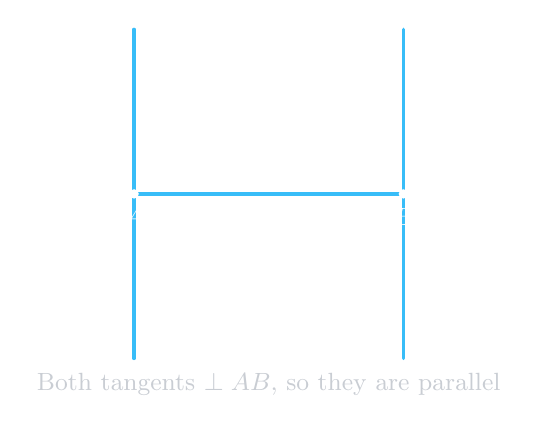
\begin{tikzpicture}[scale=0.95]
  \def\r{1.8}
  \coordinate (O) at (0,0);
  \coordinate (A) at (-\r,0);
  \coordinate (B) at (\r,0);
  \draw[base] (O) circle (\r);
  \draw[new] (A)--(B);
  \draw[new] (-\r,-2.2) -- (-\r,2.2); % tangent at A
  \draw[new] ( \r,-2.2) -- ( \r,2.2); % tangent at B
  \node[dot,label={[lab]below:$A$}] at (A) {};
  \node[dot,label={[lab]below:$B$}] at (B) {};
  \node[labm] at (0,-2.55) {Both tangents $\perp AB$, so they are parallel};
\end{tikzpicture}
\end{StepDiagram}

\Step{2} Their separation equals the diameter: $2r=2(3.5)=7$ cm.

\begin{StepDiagram}

\begin{tikzpicture}[scale=0.95]
  \def\r{1.8}
  \coordinate (O) at (0,0);
  \coordinate (A) at (-\r,0);
  \coordinate (B) at (\r,0);
  \draw[base] (O) circle (\r);
  \draw[new] (-\r,-2.2) -- (-\r,2.2);
  \draw[new] ( \r,-2.2) -- ( \r,2.2);
  \draw[help,<->] (-\r,-2.55) -- (\r,-2.55);
  \node[lab, fill=pairbg, inner sep=1.2pt] at (0,-2.55) {$7$};
\end{tikzpicture}
\end{StepDiagram}

\[
\boxed{\textcolor{green}{(b)\ 7\text{ cm}}}
\]
\end{QAPair}

% ============================================================
% Q1(ix)
\begin{QAPair}{Question 1 (ix)}
\textcolor{gold}{\bfseries Question:} Transverse common tangents intersect each other at:
(a) $1$ point \ (b) $2$ points \ (c) $3$ points \ (d) $4$ points.
\tcblower
\textcolor{green}{\bfseries Answer:}\par

\Step{1} The two transverse (internal) common tangents meet at one point.

\begin{StepDiagram}
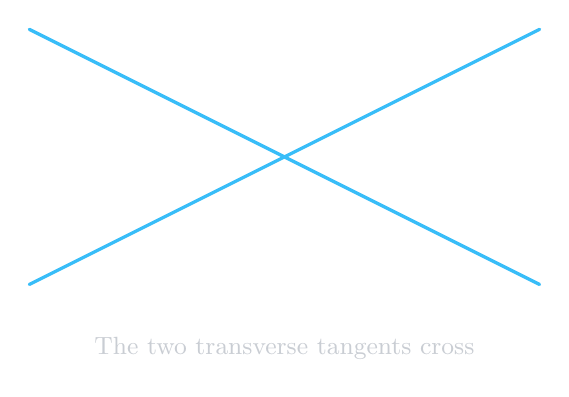
\begin{tikzpicture}[scale=0.9]
  \def\r{1.2}
  \coordinate (O1) at (-2.2,0);
  \coordinate (O2) at ( 2.2,0);
  \draw[base] (O1) circle (\r);
  \draw[base] (O2) circle (\r);
  % internal tangents (schematic)
  \draw[new] (-3.6, 1.8) -- (3.6,-1.8);
  \draw[new] (-3.6,-1.8) -- (3.6, 1.8);
  \node[labm] at (0,-2.7) {The two transverse tangents cross};
\end{tikzpicture}
\end{StepDiagram}

\Step{2} Therefore they intersect at \emph{one} point.

\begin{StepDiagram}
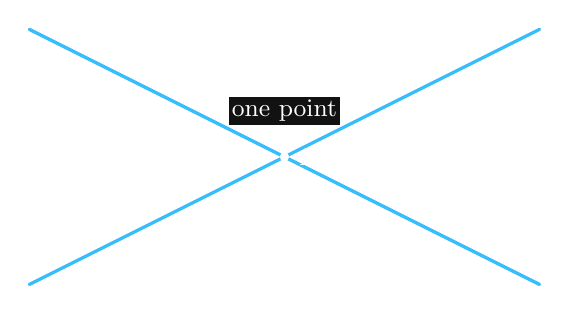
\begin{tikzpicture}[scale=0.9]
  \def\r{1.2}
  \coordinate (O1) at (-2.2,0);
  \coordinate (O2) at ( 2.2,0);
  \draw[base] (O1) circle (\r);
  \draw[base] (O2) circle (\r);
  \draw[new] (-3.6, 1.8) -- (3.6,-1.8);
  \draw[new] (-3.6,-1.8) -- (3.6, 1.8);
  \coordinate (X) at (0,0);
  \node[dot,label={[lab]right:$X$}] at (X) {};
  \node[lab, fill=pairbg, inner sep=1.2pt] at (0,0.65) {one point};
\end{tikzpicture}
\end{StepDiagram}

\[
\boxed{\textcolor{green}{(a)\ 1 point}}
\]
\end{QAPair}

% ============================================================
% Q1(x)
\begin{QAPair}{Question 1 (x)}
\textcolor{gold}{\bfseries Question:} A circle is inscribed in a square having length of side $6$ cm.
What is the radius?
(a) $24$ \ (b) $12$ \ (c) $6$ \ (d) $3$.
\tcblower
\textcolor{green}{\bfseries Answer:}\par

\Step{1} Incircle in a square has diameter equal to the side: $2r=s$.

\begin{StepDiagram}
\begin{tikzpicture}[scale=0.95]
  \coordinate (A) at (-2,-2);
  \coordinate (B) at ( 2,-2);
  \coordinate (C) at ( 2, 2);
  \coordinate (D) at (-2, 2);
  \coordinate (O) at (0,0);
  \draw[base] (A)--(B)--(C)--(D)--cycle;
  \draw[base] (O) circle (2);
  \draw[help,<->] (-2,-2.6)--(2,-2.6);
  \node[lab, fill=pairbg, inner sep=1.2pt] at (0,-2.6) {$s$};
  \node[labm] at (0,2.6) {$2r=s$};
\end{tikzpicture}
\end{StepDiagram}

\Step{2} $r=\dfrac{6}{2}=3$ cm.

\begin{StepDiagram}
\begin{tikzpicture}[scale=0.95]
  \coordinate (A) at (-2,-2);
  \coordinate (B) at ( 2,-2);
  \coordinate (C) at ( 2, 2);
  \coordinate (D) at (-2, 2);
  \coordinate (O) at (0,0);
  \draw[base] (A)--(B)--(C)--(D)--cycle;
  \draw[base] (O) circle (2);
  \node[lab, fill=pairbg, inner sep=1.2pt] at (0,0) {$r=3$};
\end{tikzpicture}
\end{StepDiagram}

\[
\boxed{\textcolor{green}{(d)\ 3}}
\]
\end{QAPair}

% ============================================================
% Q1(xi)
\begin{QAPair}{Question 1 (xi)}
\textcolor{gold}{\bfseries Question:} A square is inscribed in a circle of radius $5$ cm.
What is the length of diagonal of the square?
(a) $2.5$ cm \ (b) $5$ cm \ (c) $10$ cm \ (d) $20$ cm.
\tcblower
\textcolor{green}{\bfseries Answer:}\par

\Step{1} For an inscribed square, its diagonal equals the circle's diameter.

\begin{StepDiagram}
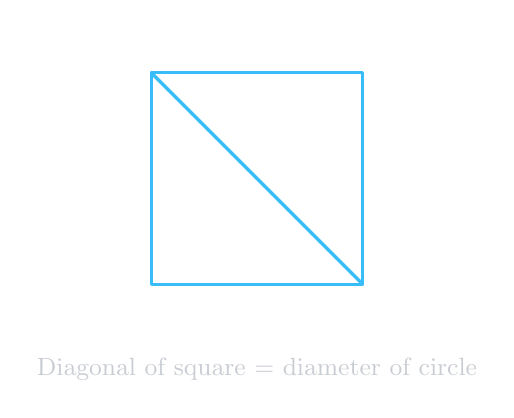
\begin{tikzpicture}[scale=0.95]
  \def\r{2.0}
  \coordinate (O) at (0,0);
  \coordinate (A) at (45:\r);
  \coordinate (B) at (135:\r);
  \coordinate (C) at (225:\r);
  \coordinate (D) at (315:\r);
  \draw[base] (O) circle (\r);
  \draw[new] (A)--(B)--(C)--(D)--cycle;
  \draw[new] (B)--(D);
  \node[labm] at (0,-2.55) {Diagonal of square = diameter of circle};
\end{tikzpicture}
\end{StepDiagram}

\Step{2} Diameter $=2r=10$ cm.

\begin{StepDiagram}
\begin{tikzpicture}[scale=0.95]
  \def\r{2.0}
  \coordinate (O) at (0,0);
  \coordinate (B) at (135:\r);
  \coordinate (D) at (315:\r);
  \draw[base] (O) circle (\r);
  \draw[new] (B)--(D);
  \node[lab, fill=pairbg, inner sep=1.2pt] at (0,0) {$10$};
\end{tikzpicture}
\end{StepDiagram}

\[
\boxed{\textcolor{green}{(c)\ 10\text{ cm}}}
\]
\end{QAPair}

% ============================================================
% Q1(xii)
\begin{QAPair}{Question 1 (xii)}
\textcolor{gold}{\bfseries Question:} Perpendicular bisectors of \dots\dots\dots always pass through centre of circle:
(a) tangents \ (b) secants \ (c) radial segments \ (d) chords.
\tcblower
\textcolor{green}{\bfseries Answer:}\par

\Step{1} The perpendicular bisector of any chord passes through the centre.

\begin{StepDiagram}
\begin{tikzpicture}[scale=1.0]
  \def\r{2.0}
  \coordinate (O) at (0,0);
  \coordinate (A) at (210:\r);
  \coordinate (B) at (330:\r);
  \coordinate (M) at ($(A)!0.5!(B)$);
  \draw[base] (O) circle (\r);
  \draw[new] (A)--(B);
  \draw[help] (M) -- ($(M)!1.4!(O)$);
  \node[dot,label={[lab]below:$O$}] at (O) {};
  \node[dot,label={[lab]below:$M$}] at (M) {};
\end{tikzpicture}
\end{StepDiagram}

\Step{2} Hence the answer is chords.

\begin{StepDiagram}
\begin{tikzpicture}[scale=1.0]
  \def\r{2.0}
  \coordinate (O) at (0,0);
  \coordinate (A) at (210:\r);
  \coordinate (B) at (330:\r);
  \coordinate (M) at ($(A)!0.5!(B)$);
  \draw[base] (O) circle (\r);
  \draw[new] (A)--(B);
  \node[lab, fill=pairbg, inner sep=1.2pt] at (0,2.35) {chord};
\end{tikzpicture}
\end{StepDiagram}

\[
\boxed{\textcolor{green}{(d)\ chords}}
\]
\end{QAPair}

% ============================================================
% Q1(xiii)
\begin{QAPair}{Question 1 (xiii)}
\textcolor{gold}{\bfseries Question:} How many circles can be drawn through three non-collinear points?
(a) infinite \ (b) $1$ \ (c) $2$ \ (d) $3$.
\tcblower
\textcolor{green}{\bfseries Answer:}\par

\Step{1} Three non-collinear points determine a unique circle.

\begin{StepDiagram}
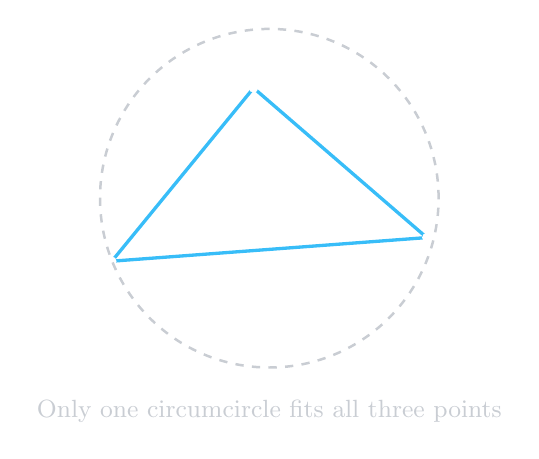
\begin{tikzpicture}[scale=1.0]
  \coordinate (A) at (-2,0);
  \coordinate (B) at (2,0.3);
  \coordinate (C) at (-0.2,2.2);
  \draw[new] (A)--(B)--(C)--cycle;
  \node[dot,label={[lab]below:$A$}] at (A) {};
  \node[dot,label={[lab]below:$B$}] at (B) {};
  \node[dot,label={[lab]above:$C$}] at (C) {};
  % simple circumcircle through 3 pts (schematic)
  \draw[help] (0,0.8) circle (2.15);
  \node[labm] at (0,-1.9) {Only one circumcircle fits all three points};
\end{tikzpicture}
\end{StepDiagram}

\Step{2} Therefore the number is $1$.

\begin{StepDiagram}
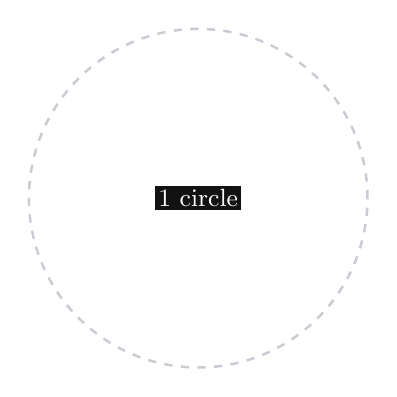
\begin{tikzpicture}[scale=1.0]
  \coordinate (A) at (-2,0);
  \coordinate (B) at (2,0.3);
  \coordinate (C) at (-0.2,2.2);
  \draw[help] (0,0.8) circle (2.15);
  \node[lab, fill=pairbg, inner sep=1.2pt] at (0,0.8) {1 circle};
\end{tikzpicture}
\end{StepDiagram}

\[
\boxed{\textcolor{green}{(b)\ 1}}
\]
\end{QAPair}

% ============================================================
% Q1(xiv)
\begin{QAPair}{Question 1 (xiv)}
\textcolor{gold}{\bfseries Question:} A circle have \dots\dots pair(s) of parallel tangents.
(a) $1$ \ (b) $2$ \ (c) $3$ \ (d) infinite.
\tcblower
\textcolor{green}{\bfseries Answer:}\par

\Step{1} For every direction, there are two opposite tangents that are parallel.

\begin{StepDiagram}
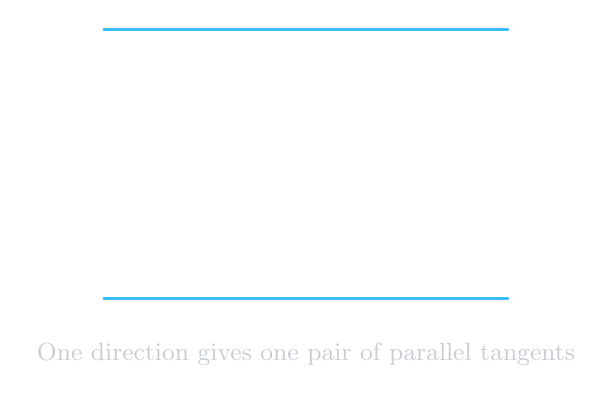
\begin{tikzpicture}[scale=0.95]
  \def\r{1.8}
  \coordinate (O) at (0,0);
  \draw[base] (O) circle (\r);
  \draw[new] (-2.7,\r) -- (2.7,\r);
  \draw[new] (-2.7,-\r) -- (2.7,-\r);
  \node[labm] at (0,-2.55) {One direction gives one pair of parallel tangents};
\end{tikzpicture}
\end{StepDiagram}

\Step{2} Since directions are infinitely many, the number of pairs is infinite.

\begin{StepDiagram}
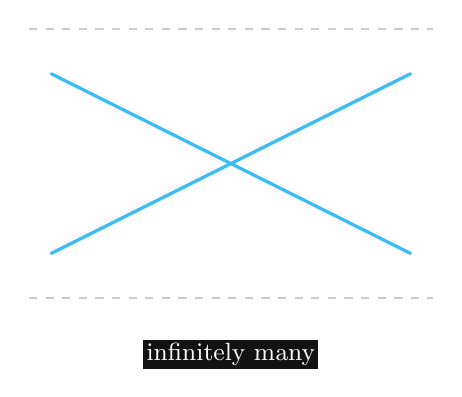
\begin{tikzpicture}[scale=0.95]
  \def\r{1.8}
  \coordinate (O) at (0,0);
  \draw[base] (O) circle (\r);
  % pair 1 (horizontal)
  \draw[help] (-2.7,\r) -- (2.7,\r);
  \draw[help] (-2.7,-\r) -- (2.7,-\r);
  % pair 2 (rotated)
  \draw[new] (-2.4, 1.2) -- (2.4,-1.2);
  \draw[new] (-2.4,-1.2) -- (2.4, 1.2);
  \node[lab, fill=pairbg, inner sep=1.2pt] at (0,-2.55) {infinitely many};
\end{tikzpicture}
\end{StepDiagram}

\[
\boxed{\textcolor{green}{(d)\ infinite}}
\]
\end{QAPair}

\end{document}
